\documentclass{beamer}
\DeclareGraphicsExtensions{.pdf,.png,.jpg,.eps}
\setbeamertemplate{caption}{\raggedright\insertcaption\par}
\title{Savings, Savings Savings}
\author{Gabriel C-Parent}
\date{IFT6751 H2015}


\usetheme{Execushares}

\begin{document}
\maketitle

\begin{frame}
\frametitle{Overview}
\begin{itemize}
	\item cvrp problem
	\item construction procedure
	\item improvement procedures
	\item genetic algorithm
	\item tabu search
	\item implementation details
	\item QA
\end{itemize}
\end{frame}


\section{The Problem}

\begin{frame}
\frametitle{Capacitated Vehicle Routing}
\begin{center}

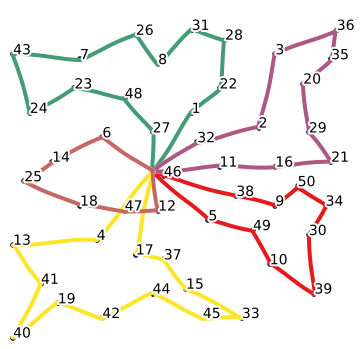
\includegraphics[scale=0.37]{figs/cvrp}


\begin{equation*}
\begin{aligned}
& \text{minimize}
& & \sum\limits_{route \in solution} distance(route) \\
& \text{subject to}
& & weight(route) \leq vehicle\ capacity
\end{aligned}
\end{equation*}

\end{center}
\end{frame}




\section{Construction}


\subsection{Random Savings}

\subsection{General Concepts}
\begin{frame}
\frametitle{Random Savings Definition}
\begin{itemize}
	\item variant of parallel savings
	\item at each iteration select randomly from top $k$ best savings
	\item $k$=1 $\rightarrow$ normal parallel savings
\end{itemize}
\end{frame}


\subsection{Results}
\begin{frame}
\frametitle{Random Savings, k=5}
\begin{center}
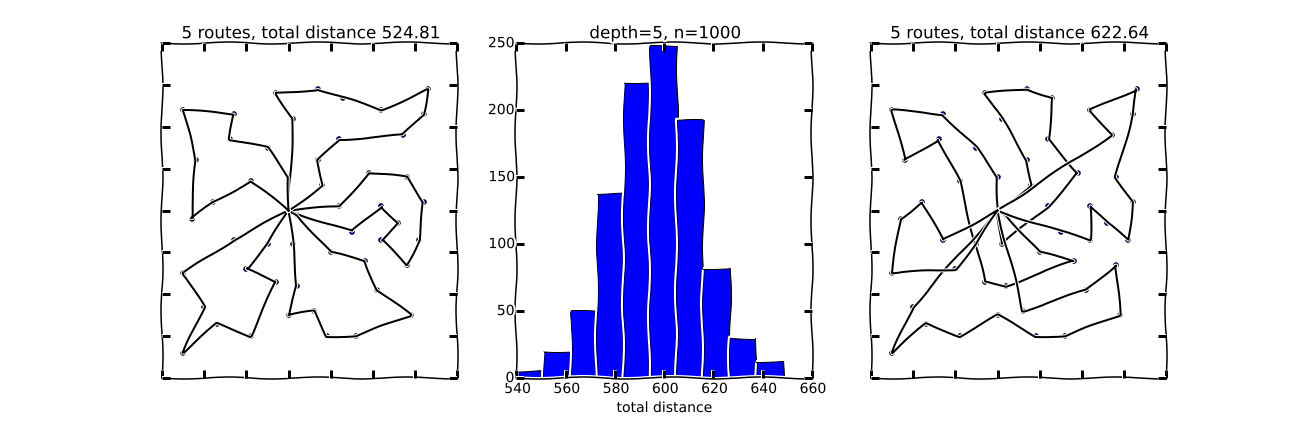
\includegraphics[scale=0.25]{figs/random_savings5}

\end{center}
\end{frame}


\begin{frame}
\frametitle{Random Savings, k=10}
\begin{center}
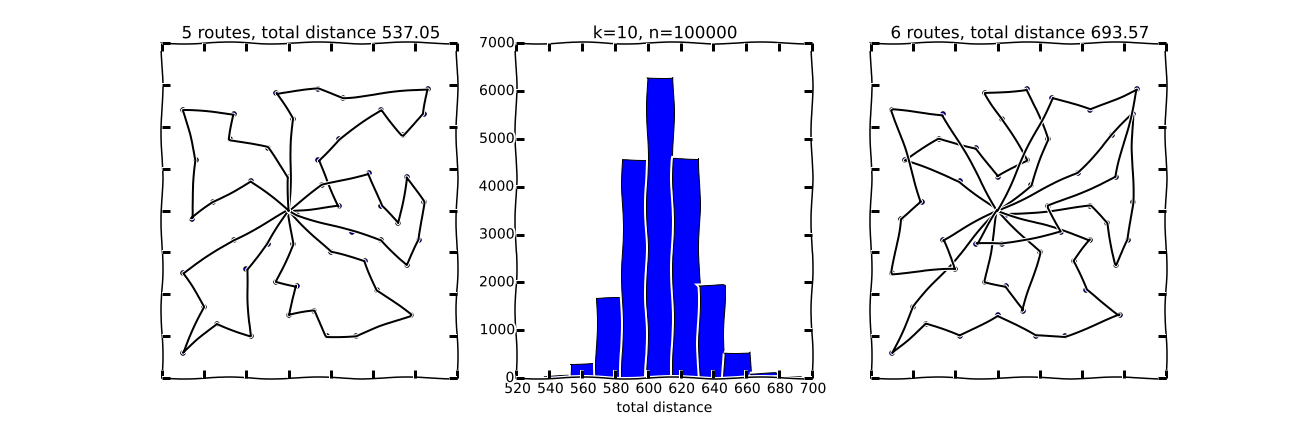
\includegraphics[scale=0.25]{figs/random_savings10}

\end{center}
\end{frame}


\begin{frame}
\frametitle{Best result in a minute}
\begin{center}
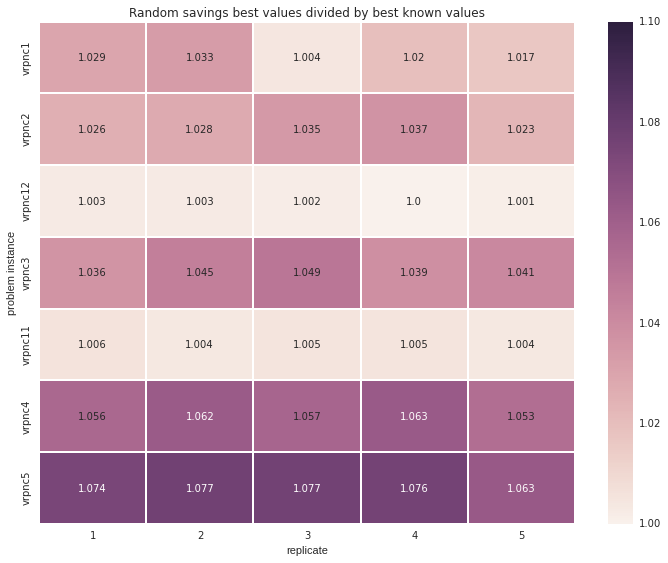
\includegraphics[scale=0.25]{figs/rs_best}

\end{center}
\end{frame}

\section{Improvement}
\subsection{2-opt descent (TSP)}

\begin{frame}
\frametitle{2-opt descent}
\begin{itemize}
	\item uses common 2-opt operator
	\item calculates all possible 2-opt for each iteration
	\item chooses the best available
\end{itemize}
\end{frame}

\begin{frame}
\frametitle{Example}
\begin{center}
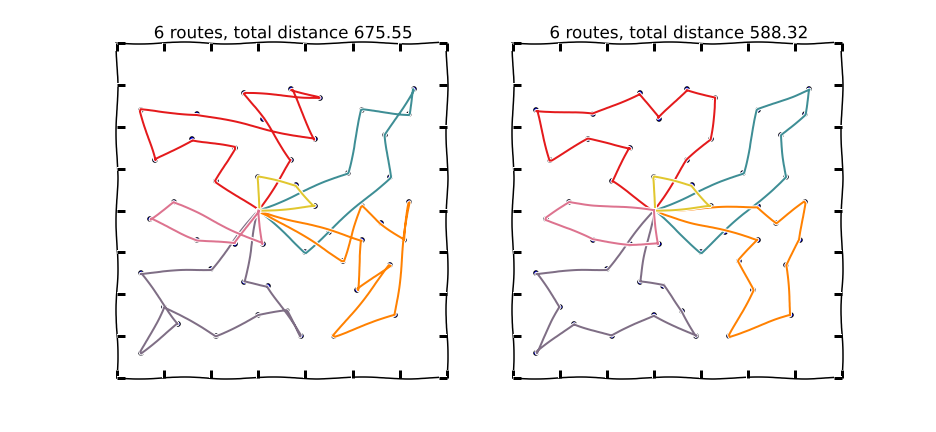
\includegraphics[scale=0.4]{figs/2opt}

\end{center}
\end{frame}


\subsection{$\lambda_1$-interchange descent}

\begin{frame}
\frametitle{$\lambda_1$-interchange definition}
\begin{itemize}
	\item exchange of customers between routes
	\item insertion (1, 0) and (0, 1) or interchange (1, 1)
	\item chooses the best option at each iteration
	\item apply 2-opt descent on routes implicated
\end{itemize}
\end{frame}


\begin{frame}
\frametitle{Example}
\begin{center}
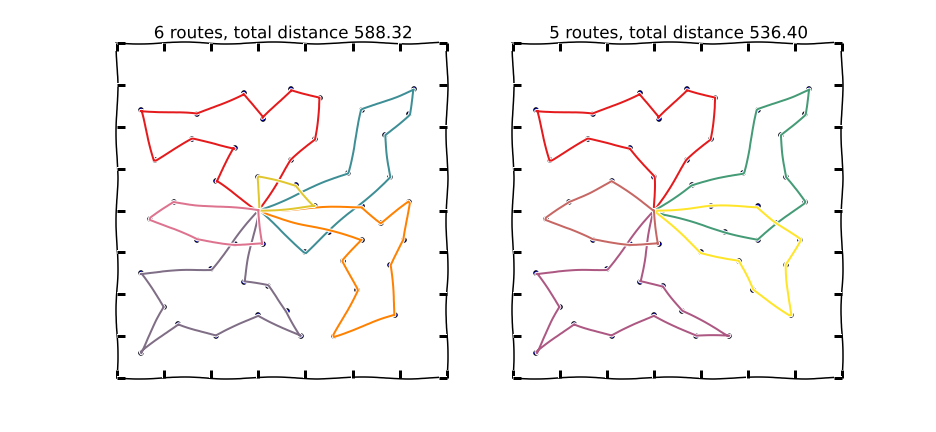
\includegraphics[scale=0.4]{figs/lambda}

\end{center}
\end{frame}

\section{Genetic Algorithm}

\subsection{Crossover}
\begin{frame}
\frametitle{Crossover}
\begin{center}
\end{center}
\end{frame}

\subsubsection{Selection of Inherited Routes}
\begin{frame}
\frametitle{Selection}
\begin{center}
\end{center}
\end{frame}

\subsubsection{Assigning Routes to Remaining Clients}
\begin{frame}
\frametitle{}
\begin{center}
\end{center}
\end{frame}

\subsection{Mutation}
\begin{frame}
\frametitle{Mutation}
\begin{center}
\end{center}
\end{frame}

\subsection{Free Parameters}
\begin{frame}
\frametitle{}
\begin{center}
\end{center}
\end{frame}

\subsection{Results}
\begin{frame}
\frametitle{Results}
\begin{center}
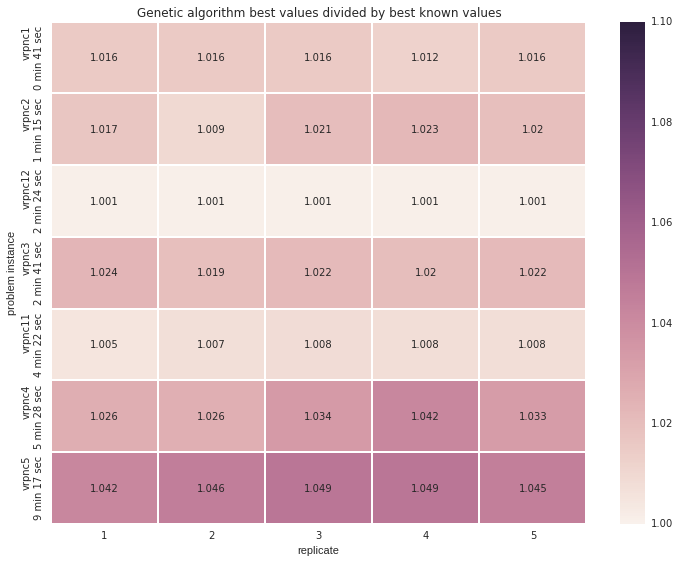
\includegraphics[scale=0.25]{figs/ga_best}

\end{center}
\end{frame}

\section{Tabu Search}

\begin{frame}
\frametitle{Results}
\begin{center}
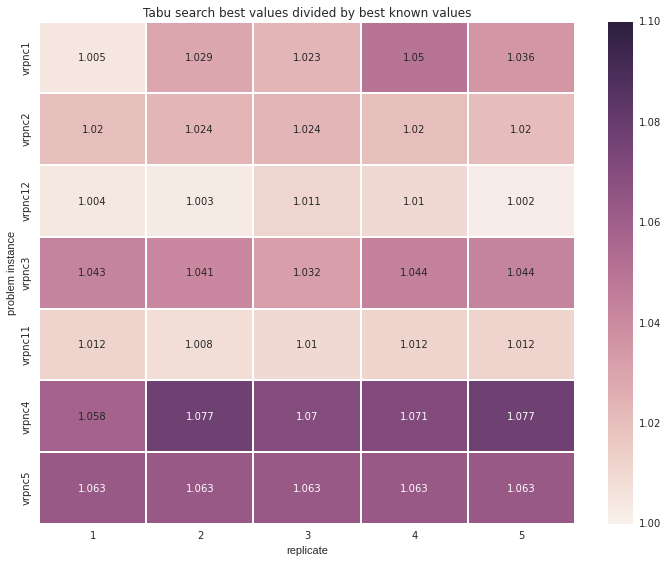
\includegraphics[scale=0.25]{figs/tabu_search}

\end{center}
\end{frame}

\section{Implementation}

\begin{frame}
\frametitle{Implementation Details}
\begin{center}

\includegraphics[scale=0.4]{figs/tools}

\end{center}
\end{frame}

\section{Results}
\begin{frame}
\frametitle{}
\begin{center}
\end{center}
\end{frame}


\section{QA}
\begin{frame}
\frametitle{QA}
\begin{center}
%\includegraphics[scale=0.4]{figs/applause}
\end{center}
\end{frame}

\end{document}